\chapter{Kameramodelle}
\label{sec:CameraModels}


Die folgenden Kapitel 2 bis 5 sollen die theoretischen Grundlagen für die bevorstehende Stereobildanalyse bilden. Im jetzigen Kapitel wird das Kameramodell vorgestellt. Des Weiteren wird die Notwendigkeit der klaren Differenzierung zwischen den einzelnen im Modell verwendeten Koordinatensysteme aufgezeigt. Sie werden dazu benötigt um zu zeigen wie später die Zusammenhänge im Weltkoordinatensystem gerechnet werden. Im Kapitel \nameref{sec:basisTransformation} wird dann aufgezeigt, wie der Wechsel zwischen den Koordinatensystemen funktioniert und wie Punkte bezüglich unterschiedlich definierter Koordinatensysteme dargestellt werden. Dies bildet den Übergang zu den darauf folgenden Kameratransformationen durch die jeweiligen Kameramatrix und Transformationsmatrx der Kameras, welche die Grundbausteine der gesamten Projektionsmatrix bilden. Im darauf foglenden Kapitel \nameref{sec:homographien}, wird zum einen gezeigt wie sich Bildpunkte, welche sich auf einer Ebene befinden, ohne bekannte Projektionsmatrizen ineinander überführen lassen. Homographien werden in dieser Arbeit eingeführt, da das Prinzip hinter deren Funktion vor allem im Kapitel \nameref{sec:rectification} bekannt sein sollte, um die Vorgehensweise dessen zu verstehen. Des weiteren bildet vor allem der geometrische Aufbau von Homographien eine gute Überleitung zu den für die Stereobildanalyse wichtigen Epipolargeometrie. Die Epipolargeometrie ist das ausschlaggebende Element, wenn es um die Kalibrierung der extrinsischen Kameraparameter und der darauf folgenden Szenenrekonstruktion geht. Sie beschreibt eine intrinsische projektive Geometrie zwischen zwei Bildern und ist insbesondere für die Korrespondenzanalyse zwischen den Punkten der Bilder ausschlaggebend.\\

(Übergang??)
Um visulle Daten aufzunehmen bedarf es optischen Geräten wie Kamera, Laser oder Sensoren. Die Geräte bilden die Dreidimensionale Welt auf eine Zweidimensionale Bildebene ab. Diese Abbildung lässt sich mithilfe von Kameramodellen beschreiben. Ein häufig benutztes Kameramodell is das Lochkameramodell. 
Das Modell beruht ausschließlich auf der geometrischen Optik und vernachlässigt physikalische Effekte wie Beugung oder die Auswirkung der Linse\cite{Heipke}. In diesem Modell, werden die Punkte im 3D-Raum durch eine sogenannte Zentralprojektion auf die Bildebene projiziert und anders herum\cite{CamerModels.,HZ}. 
%
%Als Kameramodell wird der rechnerische Prozess genannte, welcher Objekte aus dem 3D-Raum auf ein ein 2D-Bild projiziert und andersherum\cite{CamerModels.,HZ}. 
%
%Das einfachste Kameramodell ist das Lochkameramodell. Die Reduktion einer Dreidimensionalen Welt in ein Zweidimensionales Bild, ist ein Prozess bei welchem durch eine, in den meisten Fällen angewandte, Zentralprojektion eine Dimension verloren geht\cite{HZ}.
Bei einer Zentralprojektion wird ein Strahl von einem Punkt im 3D-Raum durch das Projektionszentrum der Kamera gezogen. Das Projektionszentrum der Kamera beschreibt den Punkt in der Kamera an welchem sich alle Strahlen treffen. Ein Strahl der durch einen Punkt im 3D-Raum und durch das Projektionszentrum einer Kamera geht, schneidet eine Ebene, welche im weiteren Verlauf als Bildebene bezeichnet wird. Der Schnittpunkt des Strahls mit der Bildebene wird Bildpunkt genannt \cite{CamerModels.,HZ}.\\

	\begin{minipage}{\linewidth}
	\centering
	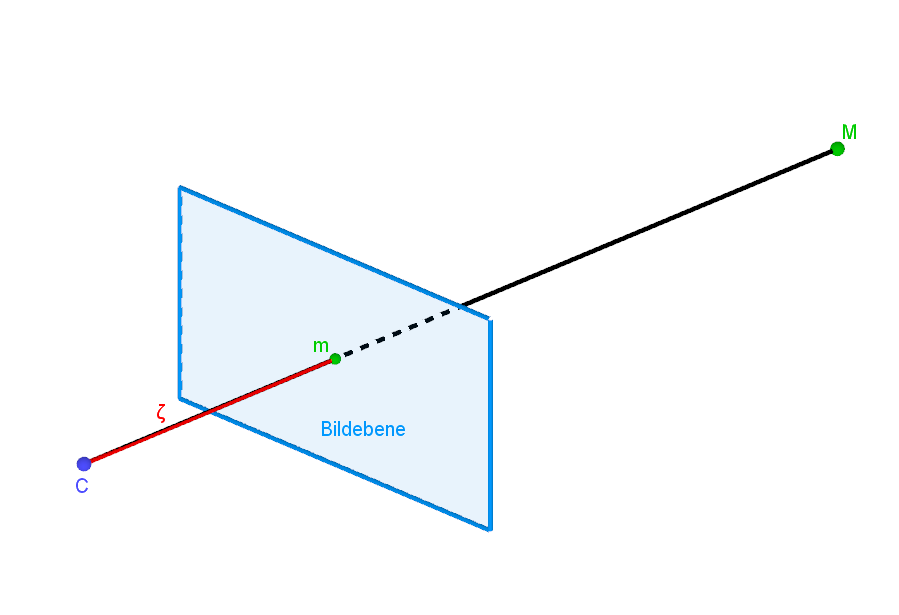
\includegraphics[width=.8\linewidth]{images/Zentralprojektion.png}
	\captionof{figure}{$C$ ist die Kamera beziehungsweise das Projektionszentrum der Kamera. In rot ist die Strecke $\zeta$ markiert. $M$ ist der Dreidimensionale Objektpunkt in Weltkoordinaten und $m$ sein projizierter Punkt auf der 2D-Bildebene}
	\label{fig:Zentralprojektion}
\end{minipage}\\ \\

\subsection{Lochkameramodell}

Das Kameramodell, auf welchem diese Arbeit aufbaut, ist das sogenannten Lochkameramodel. Es ist eines der am simpelsten aufgebauten Kameramodelle und wird standardmäßig zur Beschreibung optischer Kameras verwendet. Das Lochkameramodell beinhaltet ein Projektionszentrum $C$, welches auch gleichzeitig das Kamerazentrum bildet. Die Kamera an sich wird im Lochkameramodell als Punkt angegeben und ist meist gleichbedeutend mit dem Punkt $C$. $C$ besitzt ein eigenes Dreidimensionales Koordinatensystem, welches ab jetzt als Kamerakoordinatensystem bezeichnet wird. Das Kamerakoordinatensystem und alle weiteren Koordinatensysteme, die noch eingeführt werden, dienen dazu die Position eines Punktes innerhalb ihres geometrischen Raumes eindeutig zu bezeichnen. Das Kamerakoordinatensystem hat seinen Ursprung im Projektionszentrum $C$. Die Ausrichtung der Achsen des Koordinatensystems ist frei definierbar. Im weiteren Verlauf der Arbeit wird das Kamerakoordinatensystem als kartesisches und rechtsdrehendes Koordinatensystem definiert. In Abbildung \ref{fig:PinholeCamera3D} zeigt die X-Achse des Kamerakoordinatensystems in das Bild rein, die Y-Achse ist vertikal nach oben ausgerichtet und die Z-Achse zeigt in Richtung der Bildebene. Die Z-Achse wird hier auch als Hauptachse bezeichnet. Der Punkt in welchem sich die Hauptachse mit der Bildebene schneidet, wird Hauptpunkt $HP$ genannt. Der Abstand des Hauptpunktes zum Projektionszentrum wird im folgenden mit $\zeta$ bezeichnet und bildet einen elementaren Baustein der intrinsischen Kameraparameter. 

Der Hautpunkt $HP$ bildet den Ursprung eines neuen Zweidimensionalen Koordinatensystems, dem Bildebenenkoordinatensystem \cite{HZ}. Als vorläufig letztes Koordinatensystem wird noch ein dreidimensionales Weltkoordinatensystem eingeführt, dessen Position und Orientierung frei wählbar sind. Ein Punkt im 3D-Raum wird ab jetzt als ein Punkt in Bezug auf ein Weltkoordinatensystem bezeichnet. Des Weiteren wird der gesamte Stereoskopische Aufbau mit zwei Lochkameramodellen und den 3D-Objektpunkten im Raum immer im Bezug auf ein Weltkoordinatensystem beschrieben werden. Dieses Weltkoordinatensystem wird diesem Aufbau wiederum meist Deckungsgleich mit einem der im Stereoaufbau benutzten Kamerakoordinatensystemen gesetzt.

%(GRAFIK EINFÜGEN SIEHE HZ SEITE 8)

	\begin{minipage}{\linewidth}
	\centering
	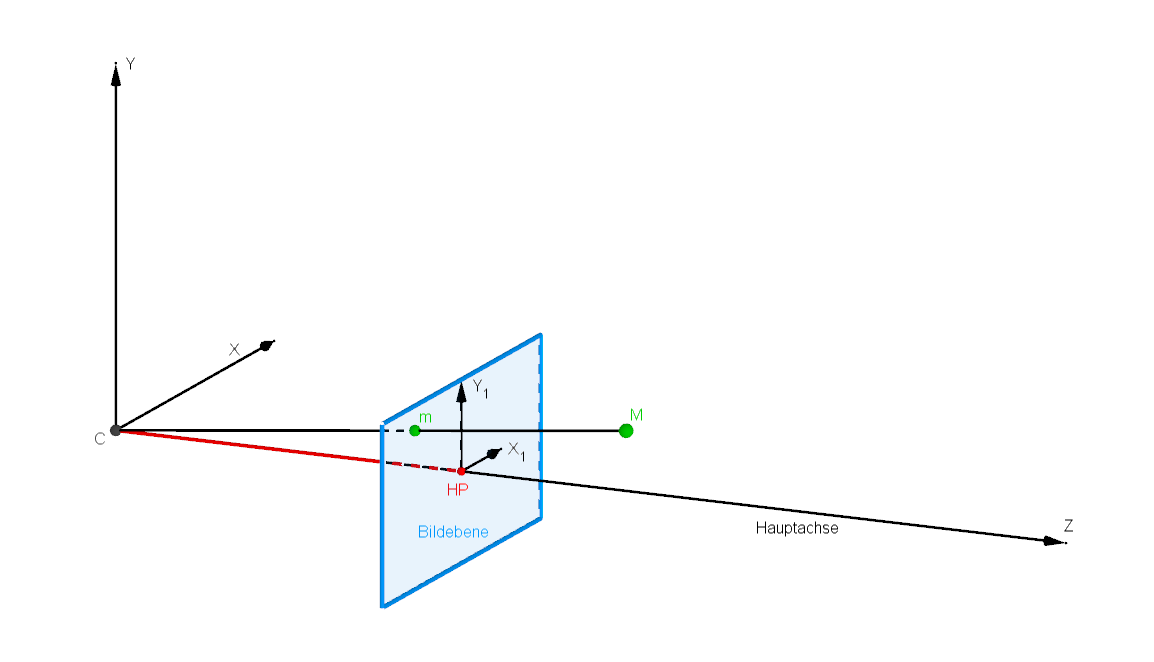
\includegraphics[width=.8\linewidth]{images/PinholeCameraModell3D.png}
	\captionof{figure}{Lochkameramodell: $C$ ist das Kamerazentrum}
	\label{fig:PinholeCamera3D}
\end{minipage}

%\begin{figure}[!htb]
%	\minipage{0.50\textwidth}
%	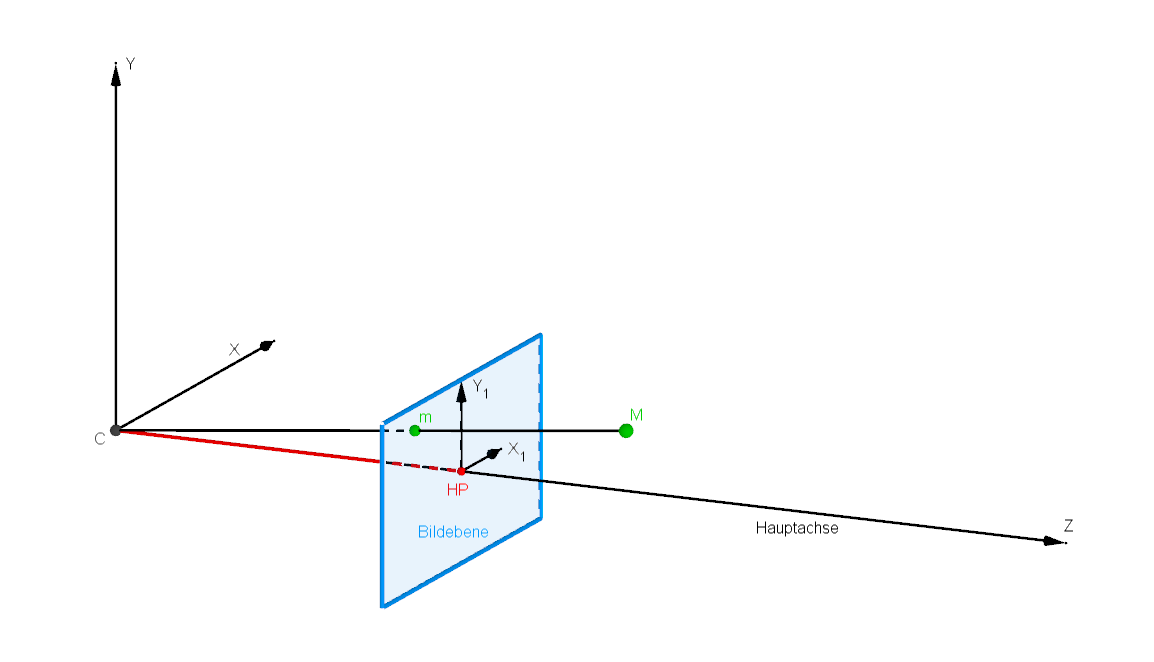
\includegraphics[width=\linewidth]{images/PinholeCameraModell3D.png}
%%	\caption{vereinfachte Top-Down-Ansicht des Szenenaufbaus des Minimalbeipspiels}
%	\label{fig:PinholeCamera}
%	\endminipage\hfill
%	\minipage{0.50\textwidth}
%	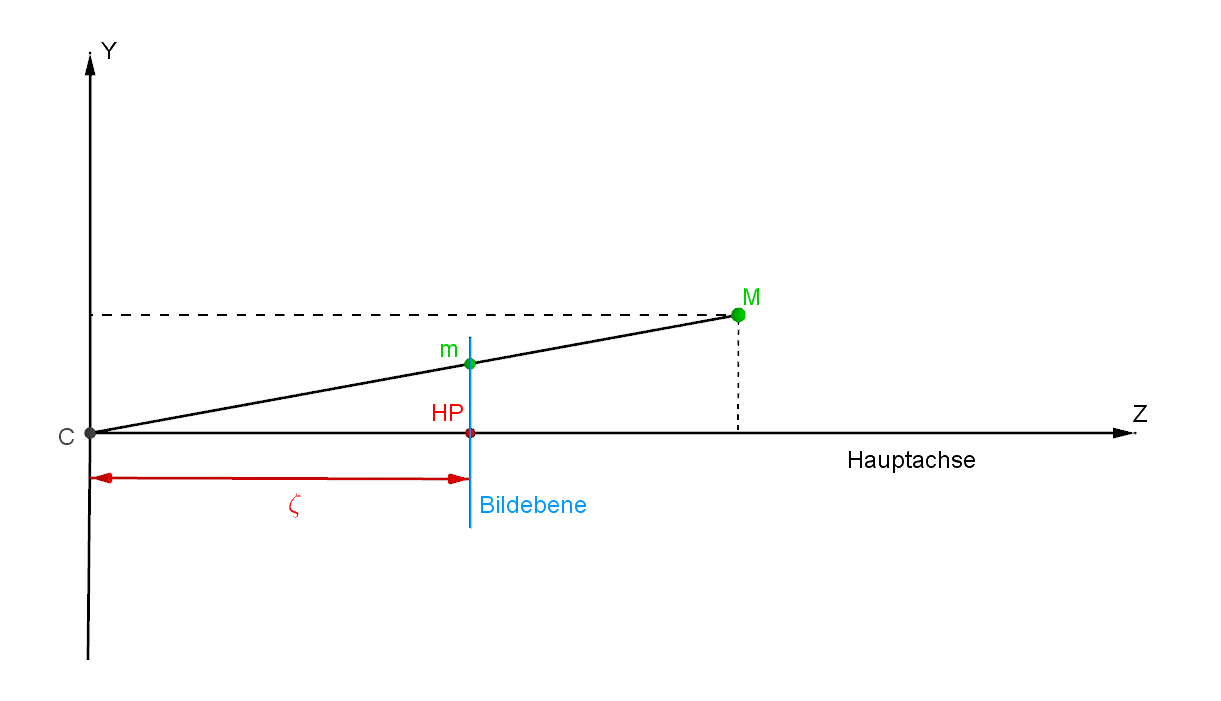
\includegraphics[width=\linewidth]{images/PinholeCameraModell2D.png}
%%	\caption{In Grün ist die Abbildung auf der Bildebenen $I$ von $C$ und in rot ist die Abbildung auf der Bildebenen $I'$ von $C'$}
%%	\label{fig:AbbildungenMinimal}
%	\endminipage\hfill	
%	\caption{Lochkameramodell}
%\end{figure}

	\begin{minipage}{\linewidth}
	\centering
	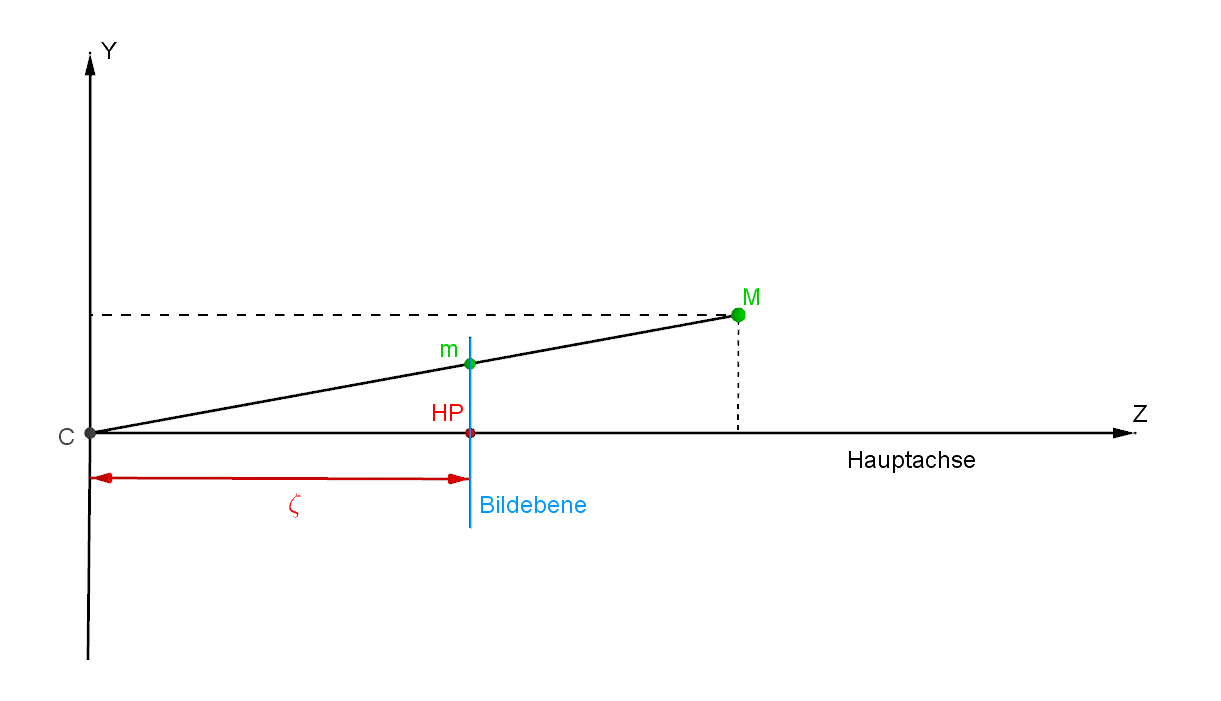
\includegraphics[width=.8\linewidth]{images/PinholeCameraModell2D.png}
	\captionof{figure}{Lochkameramodell \cite{Jianzhong}}
	\label{fig:PinholeCamera2D}
	\end{minipage}\\ \\

\subsection{Kameraparameter}

Was bedeutet nun Szenenrekonstruktion und Kamerakalibrierung eines Stereoaufbaus im Zusammenhang mit dem gerade vorgestellten Kameramodell. In Abblildung \ref{fig:StereoaufbauLochkamermodell} ist ein Stereoaufbau aus zwei Lochkameramodellen dargestellt. Jede Kamera besitzt ein eigenes Kamerakoordinatensystem und eine eigene Bildebene, welche wiederum ein eigenes Bildnebenkoordinatensystem besitzt. Des Weiteren ist ein Objektpunkt $M$ in Bezug auf ein Weltkoordinatensystem zu sehen. Die zwei Strahlen, die jeweils von $M$ ausgehen, beschreiben die Projektion des 3D-Objektpunktes $M$ auf zwei somit korrespondierende Bildpunkte $m$ und $m'$ auf den jeweiligen Bildebenen. Diese Projektion funktioniert auch in die andere Richtung. Sind zwei zueinander korrespondierende Bildpunkte auf den beiden Bildebenen gegeben, so kann jeweils ein Strahl durch die jeweiligen Projektionszentren $C$ und $C'$ und deren zugehörigen Bildebenenpunkte $m$ und $m'$ geschickt werden, welche sich dann in einem Punkt $M$ im Raum treffen. Diese umgekehrte Projektion  wird allgemein als Triangulation bezeichnet\cite{HZ}. Hier kommen jetzt die Projektionsmatrizen $P$ und $P'$ ins Spiel, welche die Projektion $M$ auf $m$ und $m'$ beschreiben mit $m = PM$ und $m' = P'M$ und genauso auch anders herum gelten für die Rückprojektion von $m$ und $m'$ auf $M$\cite{CamerModels.,HZ}.\\


	\begin{minipage}{\linewidth}
	\centering
	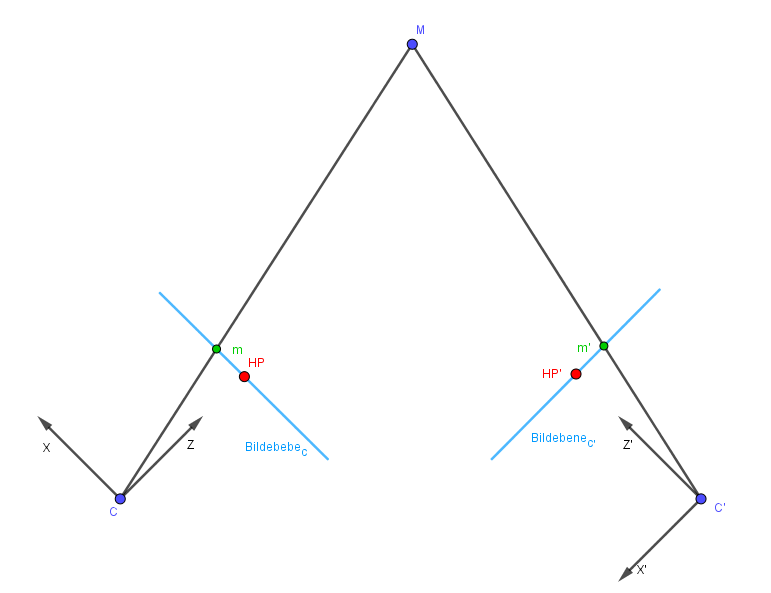
\includegraphics[width=.8\linewidth]{images/StereokopischerAufbauLochKamerModell.png}
	\captionof{figure}{Steroskopischer Aufbau mit Lochkameramodellen. Der Punkt $M$ im Raum kann mit den jeweiligen Projektionsmatrizen $P$ und $P'$ der Kameras $C$ und $C'$ in die Bildpunkte $m$ und $m'$ projiziert werden. $m=PM$ und $m'=P'M$. Eine Rückprojektion der Punkte $m$ und $m'$ zum Punkt $M$ ist mit bekannten Projektionsmatrizen genauso möglich.}
	\label{fig:StereoaufbauLochkamermodell}
\end{minipage}\\

Die Projektionsmatrizen $P$ und $P'$ bilden sich, aus den extrinsischen und intrinsischen Kameraparametern. Bei den extrinsischen Kameraparametern, handelt es sich um die jeweilige Orientierung einer Kamera bezüglich eines Weltkoordinatensystems, was in einer $3\times 4$-Transformationsmatrix $R$ beschrieben ist. $R$ kann sowohl eine Rotation als auch eine Translation beinhalten. Die intrinsischen Kameraparameter werden in der sogenannten Kameramatrix $K$ ausgedrückt. In der Literatur findet man diese wie folgt definiert\cite{HZ}.

\begin{gather}
K=\begin{bmatrix}
\alpha_x&s&x_{0}\\
0&\alpha_y&y_{0}\\
0&0&1
\end{bmatrix}
\end{gather}\\

Im folgenden werden die Elemente der Kameramatrix $K$ im erläutert. Wird nochmal von dem in Abblidung \ref{fig:PinholeCamera2D} und \ref{fig:PinholeCamera3D} beschriebenen simplen Kameramodell ausgegangen, so lässt sich ein dreidimensionaler Punkt $M$ mit $M = [X\, Y\, Z]^T$ durch aufstellen einer Matrix in einen homogenen 2D-Bildebenenpunkt $m$ mit $m = [\zeta X\, \zeta Y]^T$ projizieren.

\begin{gather}
	\begin{bmatrix}
	X\\Y\\Z
	\end{bmatrix} \mapsto
	\begin{pmatrix}
	\zeta X\\ \zeta Y\\ Z
	\end{pmatrix}
	=
	\begin{bmatrix}
	\zeta&0&0&0\\
	0&\zeta&0&0\\
	0&0&1&0
	\end{bmatrix}
	\cdot
	\begin{bmatrix}
	X\\Y\\Z
	\end{bmatrix}
	\leadsto
	\begin{pmatrix}
	\zeta \frac{X}{Z}\\ \zeta \frac{Y}{Z}
	\end{pmatrix}
\end{gather}\\

Abbildung \ref{fig:zetaErklaerung} und die Gleichungen 2.3 bis 2.5 sollen Aufschluss darüber geben, wie der Abstand $\zeta$ geometrisch zustande kommt. 

\begin{minipage}{\linewidth}
	\centering
	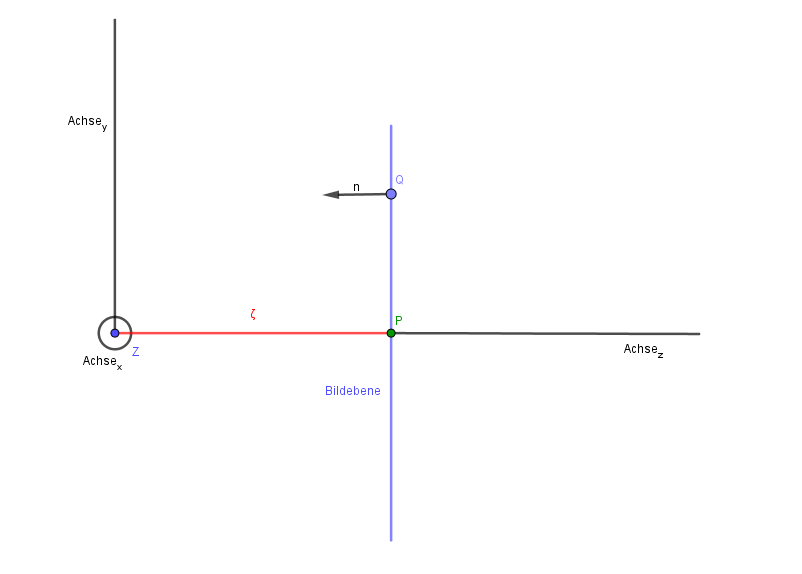
\includegraphics[width=.8\linewidth]{images/ZetaHerleitung.png}
	\captionof{figure}{In blau ist die Bildebene dargestellt auf ihr befinden sich die Punkte $Q$ und $HP$. $HP$ steht in dieser Abbildung für den Hauptpunkt. $Z$ liegt nicht auf der Ebene, Das Projetionszentrum $C$ liegt hinter der Bildebene und somit auch hinter dem Sensor. $n$ ist die Normale der Bildebene}
	\label{fig:zetaErklaerung}
\end{minipage}\\

Wie in Abbildung \ref{fig:zetaErklaerung} ersichtlich kann $\zeta$, durch folgende Gleichung ausgedrückt werden.

\begin{gather}
\vec{p}+|\vec{QZ} \cdot \vec{n}|\vec{n} = \vec{Z}
\end{gather}

$Q$ ist hierbei ein beliebigen Punkt auf der Bildebene und $\vec{n}$ der normalenvektor der Bildebene.

\begin{gather}
\vec{QZ} \cdot \hat{n} = \zeta\\
\vec{p}= \vec{Z}\zeta \hat{n}
\end{gather}

Bestimmt man nun, dass die Hauptachse $= \hat{n}$ ist, kann daraus geschlossen werden, dass $\vec{p} = \vec{Z} - \zeta \hat{n}$.


%Um die Kameramatrix allgemeiner zu formulieren und die Bedeutung hinter $\zeta$ und dessen Zusammenhang mit dem in der Literatur benutzten $f$ genauer zu erläutern, wird die Kameramatrix der Photogrammetrie in Bezug auf ein Lochkameramodell hier noch einmal genauer betrachtet und mit dem hergeleiteten Modell verglichen\cite{HZ,Heipke}. Angenommen es gilt $\zeta = f$, dann gilt für die Projektion von Punkten das selbe wie in Gleichung 2.49 nur mit $f$ statt $\zeta$. 
%
%\begin{gather}
%\begin{bmatrix}
%X\\Y\\Z\\1
%\end{bmatrix} \mapsto
%\begin{pmatrix}
%f X\\ f Y\\ Z
%\end{pmatrix}
%=
%\begin{bmatrix}
%f&0&0&0\\
%0&f&0&0\\
%0&0&1&0
%\end{bmatrix}
%\cdot
%\begin{bmatrix}
%X\\Y\\Z\\1
%\end{bmatrix}
%=
%\begin{pmatrix}
%f \frac{X}{Z}\\ f \frac{Y}{Z}\\1
%\end{pmatrix}
%\end{gather}
%
%Zum Vergleich dient die Definition im Buch von \textit{Hartley \& Zisserman}\cite{HZ}, welche der selbst hergeleiteten entspricht.
%
%
%\begin{gather}
%\begin{bmatrix}
%X\\Y\\Z\\1
%\end{bmatrix} \mapsto
%\begin{pmatrix}
%f X\\ f Y\\ Z
%\end{pmatrix}
%=
%\begin{bmatrix}
%f&0&0&0\\
%0&f&0&0\\
%0&0&1&0
%\end{bmatrix}
%\cdot
%\begin{bmatrix}
%X\\Y\\Z\\1
%\end{bmatrix}
%\end{gather}		



Die allgemeine Form der Kameramatrix bezogen auf das Lochkameramodell wird wie in Gleichung 2.1 dargestellt beschrieben. Anstelle von $f$ steht in der Kameramatrix aus Gleichung 2.1 $\alpha_x$ und $\alpha_y$. Die Werte welche $\alpha_x$ und $\alpha_y$ annehmen können, hängen von der geometrischen Form der Pixel des in der Kamera verbauten Sensors ab\cite{HZ,Photonik}.  $\alpha_x$ und $\alpha_y$ sind genau dann einheitliche Werte, wenn die Form der verbauten Pixel, ebenfalls einheitlich quadratisch ist.
 %Die Einheiten der x- und y- Achsen des Sensorkoordinatensystems sind einheitlich.  
$\alpha_x$ und $\alpha_y$ sind also genau dann ungleich, wenn die auf dem Sensor verbauten Pixel beispielsweise rechteckig oder die geometrische Form eines Parallelogramms besitzen\cite{HZ}. Im Stereoaufbau dieser Arbeit, wurden Kameras mit CMOS-Chips mit quadratischen Pixeln verwendet, weshalb $\alpha_x$ und $\alpha_y$ einheitlich sein werden. $\alpha_x$ und $\alpha_y$ entstehen aus der Multiplikation der Werte für $\zeta_x$ und $\zeta_y$ mit einem jeweiligen Skalierungsfaktor $m_x$ und $m_y$. 

In der Literatur  wird $\zeta$ meist als $f$ für \textit{focal length} bezeichnet und die Bildebene auch \textit{Focal plane} genannt \cite{HZ}. Der Begriff \textit{focal length} ist in diesem Zusammenhang jedoch etwas missverständlich. $\zeta$ sowie $f$ geben in der Kameramatrix wie sie in Gleichung 2.2 genau genommen zwei verschiedene Abstände an. Die Matrix müsste genau genommen die Form

\begin{gather*}
\begin{bmatrix}
\zeta_x&0&0&0\\
0&\zeta_y&0&0\\
0&0&1&0
\end{bmatrix}
\end{gather*}

haben. Bis jetzt war immer nur von der Bildebene die rede. Später wird jedoch auf der Bildebene noch ein weiteres zweidimensionales Koordinatensystem definiert und zwar das sogenannten Sensorkoordinatensystem. Dieses Koordinatensystem beschreibt den Aufbau des in der Kamera montierten Sensorchips. Dieser besteht meist aus einer Viereckigen Platte auf welcher sich die Pixelbausteine befinden. Diese Pixel können sowohl quadratisch, rechteckige oder auch abstrakte Formen wie ein Parallelogram haben. Das Sensorkoordinatensystem Skaliert und unterteilt seine Achsen nach den Kantenlängen der jeweiligen Pixel. Die geometrische Form dieser Pixel sind dafür verantwortlich, dass es nicht immer nur ein einheitlichen $\zeta$ geben kann. Nur wenn die Pixel quadratisch sind haben  $\zeta_x$ und $\zeta_y$ die selben Werte, sind sie beispielsweise rechteckig ändern sich dementsprechend die Werte. $\zeta_x$ und $\zeta_y$ beschreiben also genaugenommen den Abstand des Kamerazentrums zu den jeweiligen Pixelkanten.\\

(kleine Grafik??? siehe Skizze auf Block)\\ 

Sind die Pixel nicht quadratisch, wird auf die Werte $f_x$ und $f_y$ jeweils eine Skalierung $m_x$ und $m_y$ drauf multipliziert so dass  $\alpha_x = f_x \cdot m_x$ und $\alpha_y = f_y \cdot m_y$ entspricht\cite{HZ}. Die Matrixeinträge,$x_{0}$ und $y_{0}$, bilden einen Translationsvektor. Sie beinhalten die Position des Hauptpunkts auf der Bildebene. $x_{0}$ und $y_{0}$ sind definiert als $x_{0} = p_x \cdot m_x$ und $x_{0} = p_y \cdot m_y$. Der Matrixeintrag $s$ wird dem sogenannten \textit{skew-Faktor} zugeordnet, welcher nur dann zum Einsatz kommt, sollte die optische Achse nicht orthogonal auf den Bildsensor auftreffen. Sprich wenn der Chip geneigt in der Kamera montiert wurde\cite{HZ}. Die komplette Projektionsmatrix $P=KR$\cite{HZ} besteht aus der Matrixmultiplikation der hergeleiteten Transformationsmatrix $R$ welche die externen Kamerparameter repräsentiert und der Kameramatrix $K$, welche die internen Kameraparameter repräsentiert\cite{HZ,ZZGXr}.


